%   File: inclined_block_dynamics.tex
% Author: Adam Leeper
%------------------------------------------------------------------------------
%\\[0.45pc]
\providecommand{\isolatedBuild}[1]{#1}% fallback definition lets this file build normally
\isolatedBuild{
  \documentclass[11pt,letterpaper]{book}
  %\documentclass[11pt,letterpaper]{book}

% aleeper: I think these are needed for Paul's macros?
\usepackage{epsfig}
\usepackage{epstopdf}

%\makeatletter
%\typeout{The import path is \import@path}
%\makeatother

\usepackage{import}

\subimport{./}{packagesMitiguy.sty}
\subimport{./}{macrosMitiguy.tex}
\subimport{./}{PageStylesMitiguy.tex}
\subimport{./}{macrosLeeper.tex}
   % Must be found via TEXINPUTS environment variable.
  \isolatedBuildHeader{Vector Equations - Solving for Unknowns}
                      {Vector Equations - Solving for Unknowns}
\small
%
Just like with scalar equations, we can perform any valid operation to
\textbf{both sides} of a vector equation.
To solve for unknowns in a vector equation, we \textbf{dot} both sides of
the equation with any vector (though, typically a unit vector) to obtain a
scalar equation. Often, this lets us solve for an unknown directly.
If we have multiple unknowns, we can repeat this with other vectors to obtain
a set of scalar equations, which may need to be solved simultaneously.
\\[1.0pc]
\textColorBold{darkerBlue}{Dynamics of a Block on an Inclined Plane}
\\[0.45pc]
}
%%%
%%%
%%%
\begin{minipage}[t]{0.7\linewidth}
  Consider the block on a \textit{smooth} inclined plane as shown at right.
  Let system $S$ be the block.
  %
  \\[0.45pc]
  \boldUnderlineDarkRed{Draw} a FBD of $S$. State your assumptions.
  \\[0.45pc]
  \begin{minipage}[t]{0.6\linewidth}
    \vspace*{0pt}
    \Solution{}{1.0\linewidth}{
               $\bullet$ Only consider gravity from earth (down).
      \\[0.0pc]$\bullet$ Spring is linear.
      \\[0.0pc]$\bullet$ Block is modeled as a particle.
      \\[0.0pc]$\bullet$ Smooth plane has negligible friction.
      \\[0.0pc]$\bullet$ Air, thermal, and other effects negligible.
    }  % end Solution
  \end{minipage}
  \hspace{12pt}
  \begin{minipage}[t]{0.3\linewidth}
    \vspace*{0pt}
    \Solution {}{1.0\linewidth}{
      \includegraphics[width=0.9\linewidth]{blockFBD.png}
    }
\end{minipage}
%
\end{minipage}
\hfill
\begin{minipage}[t]{0.30\linewidth}
  \flushright
  \vspace*{-1.5pc}
  \includegraphics[width=0.99\linewidth]{block.png}
\end{minipage}
\\[2.0pc]
%
%
Using $\force{S} = m \accel{S}{N}$ might lead to the following vector
equation (based on assumptions about relevant forces):
%
$$-kx~\uvecx{b} \plus[\;] F_N~\uvecy{b} \minus[\;] mg~\uvecy{n}
   \equals[\;] m \ddot{x}~\uvecx{b}$$
%
\textbf{Note:} It is advantageous to express vectors in the
\boldUnderlineDarkRed{simplest} terms possible. Hence, two bases were
introduced, one aligned with the inclined plane, and one aligned with gravity,
to avoid having trig functions appear in the vector equation.
Avoiding trig functions improves efficiency and helps reduce errors.
\\[0.45pc]
%
\textbf{Given} the equation above:
\begin{enumerate}
  \item Find a scalar expression for $F_N$ (the magnitude of the ``normal
        force'' on the block from the plane).
    \\[0.45pc]
    \Solution{}{1.0\linewidth}{
      \textbf{The unknown we want is in a \uvecy{b} term, so we'll dot both
      sides with \uvecy{b}.}
      \\[0.5pc]
      \begin{tabular}{@{}r@{$\equals[\;]$}ll}
        $\uvecy{b} \cdot (-kx~\uvecx{b} \plus[\;] F_N~\uvecy{b}
        \minus[\;] mg~\uvecy{n})$ &
        $\uvecy{b} \cdot (m \ddot{x}~\uvecx{b})$
        \\[0.5pc]
        $-kx~\uvecy{b} \cdot \uvecx{b} \plus[\;] F_N~\uvecy{b} \cdot \uvecy{b}
        \minus[\;] mg~\uvecy{b} \cdot \uvecy{n}$ &
        $m \ddot{x}~\uvecy{b} \cdot \uvecx{b}$
        & $\leftarrow$ Find dot products from definition.
        \\[0.5pc]
        $ 0 \plus[\;] F_N \minus[\;] mg \cos(\theta)$ & $0$
        \\[0.5pc]
        $ F_N $ & $ mg \cos(\theta)$
      \end{tabular}
      \\[0.5pc]
    }
    \\[-0.5pc]
%
%
\item Find a scalar expression for $\ddot{x}$.
  (This is an \textbf{equation of motion} for $x$.)
  \\[0.45pc]
  \Solution{}{1.0\linewidth}{
    \textbf{The unknown we want is in a \uvecx{b} term, so we'll dot both
    sides with \uvecx{b}.}
    \\[0.5pc]
    \begin{tabular}{@{}r@{$\equals[\;]$}ll}
      $\uvecx{b} \cdot (-kx~\uvecx{b} \plus[\;] F_N~\uvecy{b} \minus[\;]
      mg~\uvecy{n})$ &
      $\uvecx{b} \cdot (m \ddot{x}~\uvecx{b})$
      \\[0.5pc]
      $-kx~\uvecx{b} \cdot \uvecx{b} \plus[\;] F_N~\uvecx{b} \cdot \uvecy{b}
      \minus[\;] mg~\uvecx{b} \cdot \uvecy{n}$ &
      $m \ddot{x}~ \uvecx{b} \cdot \uvecx{b}$ &
      $\leftarrow$ Find dot products from definition.
      \\[0.5pc]
      $ -kx \plus[\;] 0 \minus[\;] mg \sin(\theta)$ & $m\ddot{x}$
      \\[0.5pc]
      $ \ddot{x} $ & $ -\frac{k}{m}x \minus[\;] g \sin(\theta)$
    \end{tabular}
    \\[1.0pc]
  }
\end{enumerate}
%
\textbf{Note 1:} In general, it is \boldUnderlineDarkRed{not correct} to
``equate components" to create scalar equations from a vector equation.
In this example, doing so would lead to the (totally wrong) equations
$-kx = 0$, $F_N = 0$, and $-mg = 0$.
This idea is taught in calculus because it works when the directions in the
equation are mutually orthogonal, but it clearly breaks when there are non-
orthogonal vectors and/or multiple bases.
\\[1.0pc]
\textbf{Note 2:}
% In general, it is \boldUnderlineDarkRed{not efficient} to try to resolve
% vectors into components (using trig) at the vector-equation stage.
In this example, the gravity force was \boldUnderlineDarkRed{not} resolved
into \uvecx{b} and \uvecy{b} components in the vector equation.
Instead, the familiar $mg\cos(\theta)$ and $mg\sin(\theta)$ terms came
from dotting.
This is a \boldUnderlineDarkRed{key insight} to be able to do complex
and/or 3D problems efficiently. Resolving into components using trig may be
nearly impossible at times, but looking up individual dot-products in one or
more rotation tables is easy.
%(A rotation table isn't really needed in this problem).
%
\isolatedBuild {
\vfill
\end{document} }
